\documentclass{beamer}

\usepackage[utf8x]{inputenc}
\usepackage{fancyvrb}
\usepackage{color}
\usepackage{graphicx}

\usetheme{Darmstadt}

\title {High-level parallel programming in C++}
\author{Dénes Mátételki}
\institute{www.emerson.com}
\date{March 18, 2012}

\makeatletter
\def\PY@reset{\let\PY@it=\relax \let\PY@bf=\relax%
    \let\PY@ul=\relax \let\PY@tc=\relax%
    \let\PY@bc=\relax \let\PY@ff=\relax}
\def\PY@tok#1{\csname PY@tok@#1\endcsname}
\def\PY@toks#1+{\ifx\relax#1\empty\else%
    \PY@tok{#1}\expandafter\PY@toks\fi}
\def\PY@do#1{\PY@bc{\PY@tc{\PY@ul{%
    \PY@it{\PY@bf{\PY@ff{#1}}}}}}}
\def\PY#1#2{\PY@reset\PY@toks#1+\relax+\PY@do{#2}}

\def\PY@tok@gd{\def\PY@tc##1{\textcolor[rgb]{0.63,0.00,0.00}{##1}}}
\def\PY@tok@gu{\let\PY@bf=\textbf\def\PY@tc##1{\textcolor[rgb]{0.50,0.00,0.50}{##1}}}
\def\PY@tok@gt{\def\PY@tc##1{\textcolor[rgb]{0.00,0.25,0.82}{##1}}}
\def\PY@tok@gs{\let\PY@bf=\textbf}
\def\PY@tok@gr{\def\PY@tc##1{\textcolor[rgb]{1.00,0.00,0.00}{##1}}}
\def\PY@tok@cm{\let\PY@it=\textit\def\PY@tc##1{\textcolor[rgb]{0.25,0.50,0.50}{##1}}}
\def\PY@tok@vg{\def\PY@tc##1{\textcolor[rgb]{0.10,0.09,0.49}{##1}}}
\def\PY@tok@m{\def\PY@tc##1{\textcolor[rgb]{0.40,0.40,0.40}{##1}}}
\def\PY@tok@mh{\def\PY@tc##1{\textcolor[rgb]{0.40,0.40,0.40}{##1}}}
\def\PY@tok@go{\def\PY@tc##1{\textcolor[rgb]{0.50,0.50,0.50}{##1}}}
\def\PY@tok@ge{\let\PY@it=\textit}
\def\PY@tok@vc{\def\PY@tc##1{\textcolor[rgb]{0.10,0.09,0.49}{##1}}}
\def\PY@tok@il{\def\PY@tc##1{\textcolor[rgb]{0.40,0.40,0.40}{##1}}}
\def\PY@tok@cs{\let\PY@it=\textit\def\PY@tc##1{\textcolor[rgb]{0.25,0.50,0.50}{##1}}}
\def\PY@tok@cp{\def\PY@tc##1{\textcolor[rgb]{0.74,0.48,0.00}{##1}}}
\def\PY@tok@gi{\def\PY@tc##1{\textcolor[rgb]{0.00,0.63,0.00}{##1}}}
\def\PY@tok@gh{\let\PY@bf=\textbf\def\PY@tc##1{\textcolor[rgb]{0.00,0.00,0.50}{##1}}}
\def\PY@tok@ni{\let\PY@bf=\textbf\def\PY@tc##1{\textcolor[rgb]{0.60,0.60,0.60}{##1}}}
\def\PY@tok@nl{\def\PY@tc##1{\textcolor[rgb]{0.63,0.63,0.00}{##1}}}
\def\PY@tok@nn{\let\PY@bf=\textbf\def\PY@tc##1{\textcolor[rgb]{0.00,0.00,1.00}{##1}}}
\def\PY@tok@no{\def\PY@tc##1{\textcolor[rgb]{0.53,0.00,0.00}{##1}}}
\def\PY@tok@na{\def\PY@tc##1{\textcolor[rgb]{0.49,0.56,0.16}{##1}}}
\def\PY@tok@nb{\def\PY@tc##1{\textcolor[rgb]{0.00,0.50,0.00}{##1}}}
\def\PY@tok@nc{\let\PY@bf=\textbf\def\PY@tc##1{\textcolor[rgb]{0.00,0.00,1.00}{##1}}}
\def\PY@tok@nd{\def\PY@tc##1{\textcolor[rgb]{0.67,0.13,1.00}{##1}}}
\def\PY@tok@ne{\let\PY@bf=\textbf\def\PY@tc##1{\textcolor[rgb]{0.82,0.25,0.23}{##1}}}
\def\PY@tok@nf{\def\PY@tc##1{\textcolor[rgb]{0.00,0.00,1.00}{##1}}}
\def\PY@tok@si{\let\PY@bf=\textbf\def\PY@tc##1{\textcolor[rgb]{0.73,0.40,0.53}{##1}}}
\def\PY@tok@s2{\def\PY@tc##1{\textcolor[rgb]{0.73,0.13,0.13}{##1}}}
\def\PY@tok@vi{\def\PY@tc##1{\textcolor[rgb]{0.10,0.09,0.49}{##1}}}
\def\PY@tok@nt{\let\PY@bf=\textbf\def\PY@tc##1{\textcolor[rgb]{0.00,0.50,0.00}{##1}}}
\def\PY@tok@nv{\def\PY@tc##1{\textcolor[rgb]{0.10,0.09,0.49}{##1}}}
\def\PY@tok@s1{\def\PY@tc##1{\textcolor[rgb]{0.73,0.13,0.13}{##1}}}
\def\PY@tok@sh{\def\PY@tc##1{\textcolor[rgb]{0.73,0.13,0.13}{##1}}}
\def\PY@tok@sc{\def\PY@tc##1{\textcolor[rgb]{0.73,0.13,0.13}{##1}}}
\def\PY@tok@sx{\def\PY@tc##1{\textcolor[rgb]{0.00,0.50,0.00}{##1}}}
\def\PY@tok@bp{\def\PY@tc##1{\textcolor[rgb]{0.00,0.50,0.00}{##1}}}
\def\PY@tok@c1{\let\PY@it=\textit\def\PY@tc##1{\textcolor[rgb]{0.25,0.50,0.50}{##1}}}
\def\PY@tok@kc{\let\PY@bf=\textbf\def\PY@tc##1{\textcolor[rgb]{0.00,0.50,0.00}{##1}}}
\def\PY@tok@c{\let\PY@it=\textit\def\PY@tc##1{\textcolor[rgb]{0.25,0.50,0.50}{##1}}}
\def\PY@tok@mf{\def\PY@tc##1{\textcolor[rgb]{0.40,0.40,0.40}{##1}}}
\def\PY@tok@err{\def\PY@bc##1{\fcolorbox[rgb]{1.00,0.00,0.00}{1,1,1}{##1}}}
\def\PY@tok@kd{\let\PY@bf=\textbf\def\PY@tc##1{\textcolor[rgb]{0.00,0.50,0.00}{##1}}}
\def\PY@tok@ss{\def\PY@tc##1{\textcolor[rgb]{0.10,0.09,0.49}{##1}}}
\def\PY@tok@sr{\def\PY@tc##1{\textcolor[rgb]{0.73,0.40,0.53}{##1}}}
\def\PY@tok@mo{\def\PY@tc##1{\textcolor[rgb]{0.40,0.40,0.40}{##1}}}
\def\PY@tok@kn{\let\PY@bf=\textbf\def\PY@tc##1{\textcolor[rgb]{0.00,0.50,0.00}{##1}}}
\def\PY@tok@mi{\def\PY@tc##1{\textcolor[rgb]{0.40,0.40,0.40}{##1}}}
\def\PY@tok@gp{\let\PY@bf=\textbf\def\PY@tc##1{\textcolor[rgb]{0.00,0.00,0.50}{##1}}}
\def\PY@tok@o{\def\PY@tc##1{\textcolor[rgb]{0.40,0.40,0.40}{##1}}}
\def\PY@tok@kr{\let\PY@bf=\textbf\def\PY@tc##1{\textcolor[rgb]{0.00,0.50,0.00}{##1}}}
\def\PY@tok@s{\def\PY@tc##1{\textcolor[rgb]{0.73,0.13,0.13}{##1}}}
\def\PY@tok@kp{\def\PY@tc##1{\textcolor[rgb]{0.00,0.50,0.00}{##1}}}
\def\PY@tok@w{\def\PY@tc##1{\textcolor[rgb]{0.73,0.73,0.73}{##1}}}
\def\PY@tok@kt{\def\PY@tc##1{\textcolor[rgb]{0.69,0.00,0.25}{##1}}}
\def\PY@tok@ow{\let\PY@bf=\textbf\def\PY@tc##1{\textcolor[rgb]{0.67,0.13,1.00}{##1}}}
\def\PY@tok@sb{\def\PY@tc##1{\textcolor[rgb]{0.73,0.13,0.13}{##1}}}
\def\PY@tok@k{\let\PY@bf=\textbf\def\PY@tc##1{\textcolor[rgb]{0.00,0.50,0.00}{##1}}}
\def\PY@tok@se{\let\PY@bf=\textbf\def\PY@tc##1{\textcolor[rgb]{0.73,0.40,0.13}{##1}}}
\def\PY@tok@sd{\let\PY@it=\textit\def\PY@tc##1{\textcolor[rgb]{0.73,0.13,0.13}{##1}}}

\def\PYZbs{\char`\\}
\def\PYZus{\char`\_}
\def\PYZob{\char`\{}
\def\PYZcb{\char`\}}
\def\PYZca{\char`\^}
\def\PYZsh{\char`\#}
\def\PYZpc{\char`\%}
\def\PYZdl{\char`\$}
\def\PYZti{\char`\~}
% for compatibility with earlier versions
\def\PYZat{@}
\def\PYZlb{[}
\def\PYZrb{]}
\makeatother

\begin{document}

%----------- slide --------------------------------------------------%

\begin{frame}
\titlepage
\end{frame}

%----------- slide --------------------------------------------------%

\begin{frame}
\frametitle{Table of contents}
\tableofcontents
\end{frame}

\section{Theory}

\subsection{High level vs. low level}

%----------- slide --------------------------------------------------%

\begin{frame}{Comparison}
\begin{columns}[t]
\column{1.5in}

\begin{block}{High level}
\small 
\begin{itemize}
  \item Auto scaling-up
  \item Threadpool handling, load balancing.
  \item Synchronization and mutexes are handled.
\end{itemize}
\end{block}

\column{1.5in}

\begin{block}{Low level}
\small
\begin{itemize}
  \item Manual thread creation.
  \item Manual joins and mutex handling.
  \item Better for event and I/O based threading.
  \item Compiler and external library independend.
\end{itemize}
\end{block}

\end{columns}
\end{frame}

%----------- slide --------------------------------------------------%

\begin{frame}{Compared softwares (performance, code complexity)}
\begin{columns}[t]
\column{1.5in}

\begin{block}{Used}
\small
\begin{itemize}
  \item Standard c++ (serial examples)
  \item openMP\cite{openmp}
  \item Intel Thread Building Blocks (TBB)\cite{itbb}
  \item QtConcurrent\cite{qtconcurrent}
\end{itemize}
\end{block}

\column{1.5in}

\begin{block}{Skipped}
\small
\begin{itemize}
  \item std::thread, std::mutex (c++0x)\cite{cpp_thread}
  \item POSIX threads\cite{posix_threads}
  \item QThread\cite{qt_thread}
\end{itemize}
\end{block}

\end{columns}


\begin{exampleblock}{Co-existence\cite{itbb_openmp_nativethreads}}
\small
Possible, but the separate threadpools can lead to oversubscription.
\end{exampleblock}

\end{frame}

%----------- slide --------------------------------------------------%

\begin{frame}{Comparison}

\begin{columns}[t]
\column{1.5in}

\begin{block}{openMP}
\small 
\begin{itemize}
  \item Compiler support needed.
  \item C, C++, fortran.
  \item Best for bounded loops.
  \item No need for big code re-write.
  \item Hard to debug.
  \item Managed by a non-profit organization.
\end{itemize}
\end{block}
\column{1.5in}


\begin{block}{Intel TBB}
\small
\begin{itemize}
  \item Object oriented.
  \item Concurrent data types.
  \item Parallel algorithms.
  \item Work stealing: dynamic load sharing.
  \item Relies heavily on templates.
  \item Heavy code rewrite is needed.
\end{itemize}
\end{block}

\column{1.5in}

\begin{block}{QtConcurrent}
\small
\begin{itemize}
  \item Object oriented
  \item Limited number of algorithms.
  \item ...
\end{itemize}
\end{block}

\end{columns}

\end{frame}


\subsection{Algorithms}

%----------- slide --------------------------------------------------%

\begin{frame}[fragile]{Used algorithms for testing}

\begin{block}{List}
\begin{itemize}
  \item Map - Applies a given function to each element of a container.
  \item Reduction - Combines the results of sub-parts.
  \item Sort - Puts elements of a list in a certain order.
\end{itemize}
\end{block}

\begin{exampleblock}{Note}
\small
\begin{itemize}
  \item The used container is an \verb|std::vector<float>|
  \item Container size was 60 million with random floats [1, 1000]
  \item Execution times are the avareges of 3 executions.
  \item Used hardware was an Intel Xeon 64-bit machine with 6 cores (12 threads), 3,4Mz.
  \item Compiled with gcc-4.4 and use flags: \verb|-O3| \verb|-ffast-math| \verb|-fwhole-program| 
\verb|-fomit-frame-pointer| \verb|-march=native| \verb|-m64|
\end{itemize}
\end{exampleblock}
      

\end{frame}


\section{Code samples}

\subsection{Map}

%----------- slide --------------------------------------------------%

\begin{frame}[fragile]{Serial map}

\begin{block}{c++ code}

\tiny
\begin{Verbatim}[commandchars=\\\{\},numbers=left,firstnumber=1,stepnumber=1]
\PY{k+kt}{float} \PY{n}{modify}\PY{p}{(}\PY{k+kt}{float} \PY{n}{value}\PY{p}{)}
\PY{p}{\PYZob{}}
  \PY{k}{return} \PY{l+m+mf}{13.37} \PY{o}{*} \PY{n}{pow}\PY{p}{(}\PY{n}{sqrt}\PY{p}{(}\PY{n}{value}\PY{p}{)}\PY{p}{,} \PY{n}{log}\PY{p}{(}\PY{n}{value}\PY{p}{)}\PY{p}{)}\PY{p}{;}
\PY{p}{\PYZcb{}}


\PY{k+kt}{void} \PY{n}{serialMap}\PY{p}{(}\PY{n}{std}\PY{o}{:}\PY{o}{:}\PY{n}{vector}\PY{o}{<}\PY{k+kt}{float}\PY{o}{>}\PY{o}{&} \PY{n}{data}\PY{p}{)}
\PY{p}{\PYZob{}}
  \PY{k}{for} \PY{p}{(}\PY{n}{size\PYZus{}t} \PY{n}{i} \PY{o}{=} \PY{l+m+mi}{0}\PY{p}{;} \PY{n}{i} \PY{o}{<} \PY{n}{data}\PY{p}{.}\PY{n}{size}\PY{p}{(}\PY{p}{)}\PY{p}{;} \PY{n}{i}\PY{o}{+}\PY{o}{+}\PY{p}{)}
    \PY{n}{modify}\PY{p}{(}\PY{n}{data}\PY{p}{[}\PY{n}{i}\PY{p}{]}\PY{p}{)}\PY{p}{;}
\PY{p}{\PYZcb{}}
\end{Verbatim}
\end{block}

\begin{exampleblock}{Note}
  \small
  \begin{itemize}
    \item ``chunksize'' equals the size of the data.
    \item This modify function will be used by the parallel examples too.
  \end{itemize}
\end{exampleblock}

\end{frame}

%----------- slide --------------------------------------------------%

\begin{frame}[fragile]{openMP parallel map}

\begin{block}{c++ code}

\tiny
\begin{Verbatim}[commandchars=\\\{\},numbers=left,firstnumber=1,stepnumber=1]
\PY{k+kt}{void} \PY{n}{openMpMap}\PY{p}{(}\PY{n}{std}\PY{o}{:}\PY{o}{:}\PY{n}{vector}\PY{o}{<}\PY{k+kt}{float}\PY{o}{>}\PY{o}{&} \PY{n}{data}\PY{p}{,}
               \PY{k}{const} \PY{k+kt}{int} \PY{n}{numberOfThreads}\PY{p}{,}
               \PY{k}{const} \PY{k+kt}{int} \PY{n}{chunkSize}\PY{p}{)}
\PY{p}{\PYZob{}}
  \PY{n}{size\PYZus{}t} \PY{n}{i}\PY{p}{;}

\PY{c+cp}{\PYZsh{}}\PY{c+cp}{pragma omp parallel for      \PYZbs{}}
\PY{c+cp}{  default(shared) private(i)  \PYZbs{}}
\PY{c+cp}{  schedule(dynamic, chunkSize) \PYZbs{}}
\PY{c+cp}{  num\PYZus{}threads(numberOfThreads)}

  \PY{k}{for} \PY{p}{(}\PY{n}{i} \PY{o}{=} \PY{l+m+mi}{0}\PY{p}{;} \PY{n}{i} \PY{o}{<} \PY{n}{data}\PY{p}{.}\PY{n}{size}\PY{p}{(}\PY{p}{)}\PY{p}{;} \PY{n}{i}\PY{o}{+}\PY{o}{+}\PY{p}{)}
    \PY{n}{data}\PY{p}{[}\PY{n}{i}\PY{p}{]} \PY{o}{=} \PY{n}{modify}\PY{p}{(}\PY{n}{data}\PY{p}{[}\PY{n}{i}\PY{p}{]}\PY{p}{)}\PY{p}{;}
\PY{p}{\PYZcb{}}
\end{Verbatim}

\end{block}

\begin{exampleblock}{Note}
\small
Making it run in parallel is just a single pragma line.
\end{exampleblock}

\end{frame}

%----------- slide --------------------------------------------------%


\begin{frame}[fragile]{Intel TBB map}

\begin{block}{c++ code}

\tiny
\begin{Verbatim}[commandchars=\\\{\},numbers=left,firstnumber=1,stepnumber=1]
\PY{k}{class} \PY{n+nc}{itbbMap} \PY{p}{\PYZob{}}
\PY{k}{public}\PY{o}{:}

  \PY{n}{itbbMap}\PY{p}{(}\PY{n}{std}\PY{o}{:}\PY{o}{:}\PY{n}{vector}\PY{o}{<}\PY{k+kt}{float}\PY{o}{>}\PY{o}{&} \PY{n}{data}\PY{p}{)}
    \PY{o}{:} \PY{n}{m\PYZus{}data}\PY{p}{(}\PY{n}{data}\PY{p}{)} \PY{p}{\PYZob{}}\PY{p}{\PYZcb{}}

  \PY{k+kt}{void} \PY{k}{operator}\PY{p}{(}\PY{p}{)}\PY{p}{(}\PY{k}{const} \PY{n}{tbb}\PY{o}{:}\PY{o}{:}\PY{n}{blocked\PYZus{}range}\PY{o}{<}\PY{n}{size\PYZus{}t}\PY{o}{>}\PY{o}{&} \PY{n}{r}\PY{p}{)} \PY{k}{const} \PY{p}{\PYZob{}}
    \PY{k}{for}\PY{p}{(} \PY{n}{size\PYZus{}t} \PY{n}{i} \PY{o}{=} \PY{n}{r}\PY{p}{.}\PY{n}{begin}\PY{p}{(}\PY{p}{)}\PY{p}{;} \PY{n}{i} \PY{o}{!}\PY{o}{=} \PY{n}{r}\PY{p}{.}\PY{n}{end}\PY{p}{(}\PY{p}{)}\PY{p}{;} \PY{n}{i}\PY{o}{+}\PY{o}{+} \PY{p}{)}
      \PY{n}{m\PYZus{}data}\PY{p}{[}\PY{n}{i}\PY{p}{]} \PY{o}{=} \PY{n}{modify}\PY{p}{(}\PY{n}{m\PYZus{}data}\PY{p}{[}\PY{n}{i}\PY{p}{]}\PY{p}{)}\PY{p}{;}
  \PY{p}{\PYZcb{}}

\PY{k}{private}\PY{o}{:}
  \PY{n}{std}\PY{o}{:}\PY{o}{:}\PY{n}{vector}\PY{o}{<}\PY{k+kt}{float}\PY{o}{>}\PY{o}{&} \PY{n}{m\PYZus{}data}\PY{p}{;}
\PY{p}{\PYZcb{}}\PY{p}{;}


\PY{n}{tbb}\PY{o}{:}\PY{o}{:}\PY{n}{task\PYZus{}scheduler\PYZus{}init} \PY{n}{init}\PY{p}{(}\PY{n}{NUMBER\PYZus{}OF\PYZus{}THREADS}\PY{p}{)}\PY{p}{;}
\PY{n}{itbbMap} \PY{n}{im}\PY{p}{(}\PY{n}{data}\PY{p}{)}\PY{p}{;}
\PY{n}{tbb}\PY{o}{:}\PY{o}{:}\PY{n}{parallel\PYZus{}for}\PY{p}{(}\PY{n}{tbb}\PY{o}{:}\PY{o}{:}\PY{n}{blocked\PYZus{}range}\PY{o}{<}\PY{n}{size\PYZus{}t}\PY{o}{>}\PY{p}{(}\PY{l+m+mi}{0}\PY{p}{,} \PY{n}{data}\PY{p}{.}\PY{n}{size}\PY{p}{(}\PY{p}{)}\PY{p}{,} \PY{n}{CHUNK\PYZus{}SIZE}\PY{p}{)}\PY{p}{,} \PY{n}{im}\PY{p}{)}\PY{p}{;}
\end{Verbatim}

\end{block}

\begin{exampleblock}{Note}
\small
Running a functor on chunks in parallel.
\end{exampleblock}

\end{frame}

%----------- slide --------------------------------------------------%


\begin{frame}[fragile]{QtConcurrent map}

\begin{block}{c++ code}

\tiny
\begin{Verbatim}[commandchars=\\\{\},numbers=left,firstnumber=1,stepnumber=1]
\PY{k+kt}{void} \PY{n}{QtMap}\PY{p}{(}\PY{n}{std}\PY{o}{:}\PY{o}{:}\PY{n}{vector}\PY{o}{<}\PY{k+kt}{float}\PY{o}{>}\PY{o}{&} \PY{n}{data}\PY{p}{)}
\PY{p}{\PYZob{}}
  \PY{n}{QtConcurrent}\PY{o}{:}\PY{o}{:}\PY{n}{blockingMap}\PY{p}{(}\PY{n}{data}\PY{p}{,} \PY{n}{modify}\PY{p}{)}\PY{p}{;}
\PY{p}{\PYZcb{}}

\PY{n}{QThreadPool}\PY{o}{:}\PY{o}{:}\PY{n}{globalInstance}\PY{p}{(}\PY{p}{)}\PY{o}{-}\PY{o}{>}\PY{n}{setMaxThreadCount}\PY{p}{(}\PY{n}{NUMBER\PYZus{}OF\PYZus{}THREADS}\PY{p}{)}\PY{p}{;}
\end{Verbatim}


\end{block}

\begin{exampleblock}{Note}
  \small
  \begin{itemize}
    \item Chunksize is 1.
    \item Blocks till the iterator reaches the end.
  \end{itemize}
\end{exampleblock}

\end{frame}

%----------- slide --------------------------------------------------%

\begin{frame}[fragile]{Map execution times}

\begin{center}
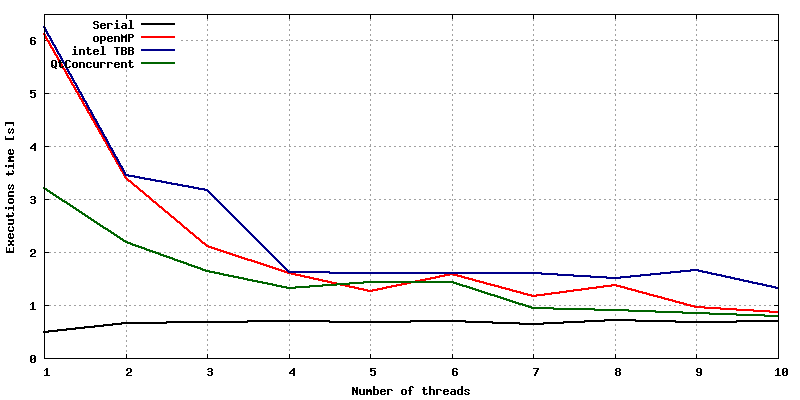
\includegraphics[height=5cm]{map.png} 
\end{center}

\begin{exampleblock}{Note}
\small
Serial remained the fastest (memory bound?) - No need to paralellize.
\end{exampleblock}

\end{frame}

\subsection{Reduce}

%----------- slide --------------------------------------------------%


\begin{frame}[fragile]{Serial reduce}

\begin{block}{c++ code}

\tiny
\begin{Verbatim}[commandchars=\\\{\},numbers=left,firstnumber=1,stepnumber=1]
\PY{k+kt}{float} \PY{n}{serialReduce}\PY{p}{(}\PY{n}{std}\PY{o}{:}\PY{o}{:}\PY{n}{vector}\PY{o}{<}\PY{k+kt}{float}\PY{o}{>}\PY{o}{&} \PY{n}{data}\PY{p}{)}
\PY{p}{\PYZob{}}
  \PY{k+kt}{float} \PY{n}{min}\PY{p}{(}\PY{n}{FLT\PYZus{}MAX}\PY{p}{)}\PY{p}{;}
  \PY{k}{for} \PY{p}{(}\PY{n}{size\PYZus{}t} \PY{n}{i} \PY{o}{=} \PY{l+m+mi}{0}\PY{p}{;} \PY{n}{i} \PY{o}{<} \PY{n}{data}\PY{p}{.}\PY{n}{size}\PY{p}{(}\PY{p}{)}\PY{p}{;} \PY{n}{i}\PY{o}{+}\PY{o}{+}\PY{p}{)}
    \PY{k}{if} \PY{p}{(}\PY{n}{data}\PY{p}{[}\PY{n}{i}\PY{p}{]} \PY{o}{<} \PY{n}{min}\PY{p}{)}
      \PY{n}{min} \PY{o}{=} \PY{n}{data}\PY{p}{[}\PY{n}{i}\PY{p}{]}\PY{p}{;}

  \PY{k}{return} \PY{n}{min}\PY{p}{;}
\PY{p}{\PYZcb{}}
\end{Verbatim}

\end{block}

\begin{exampleblock}{Note}
  \small
  \begin{itemize}
    \item Minimum value search.
    \item Not actually a reduce.
    \item Following examples will try to achive this too.
  \end{itemize}
\end{exampleblock}

\end{frame}

%----------- slide --------------------------------------------------%


\begin{frame}[fragile]{openMP reduce}

\begin{block}{c++ code}

\tiny
\begin{Verbatim}[commandchars=\\\{\},numbers=left,firstnumber=1,stepnumber=1]
\PY{k+kt}{int} \PY{n}{openMpReduce}\PY{p}{(}\PY{n}{std}\PY{o}{:}\PY{o}{:}\PY{n}{vector}\PY{o}{<}\PY{k+kt}{float}\PY{o}{>}\PY{o}{&} \PY{n}{data}\PY{p}{,}
                 \PY{k}{const} \PY{k+kt}{int} \PY{n}{numberOfThreads}\PY{p}{,}
                 \PY{k}{const} \PY{k+kt}{int} \PY{n}{chunkSize}\PY{p}{)}
\PY{p}{\PYZob{}}
  \PY{n}{size\PYZus{}t} \PY{n}{i}\PY{p}{;}
  \PY{n}{std}\PY{o}{:}\PY{o}{:}\PY{n}{vector}\PY{o}{<}\PY{k+kt}{float}\PY{o}{>} \PY{n}{separate\PYZus{}results}\PY{p}{(}\PY{n}{numberOfThreads}\PY{p}{,} \PY{n}{FLT\PYZus{}MAX}\PY{p}{)}\PY{p}{;}

\PY{c+cp}{\PYZsh{}}\PY{c+cp}{pragma omp parallel \PYZbs{}}
\PY{c+cp}{  default(shared) private(i) \PYZbs{}}
\PY{c+cp}{  num\PYZus{}threads(numberOfThreads)}
  \PY{p}{\PYZob{}}
    \PY{k+kt}{int} \PY{n}{threadId} \PY{o}{=} \PY{n}{omp\PYZus{}get\PYZus{}thread\PYZus{}num}\PY{p}{(}\PY{p}{)}\PY{p}{;}

\PY{c+cp}{\PYZsh{}}\PY{c+cp}{pragma omp for schedule(dynamic, chunkSize)}

  \PY{k}{for} \PY{p}{(}\PY{n}{i} \PY{o}{=} \PY{l+m+mi}{0}\PY{p}{;} \PY{n}{i} \PY{o}{<} \PY{n}{data}\PY{p}{.}\PY{n}{size}\PY{p}{(}\PY{p}{)}\PY{p}{;} \PY{n}{i}\PY{o}{+}\PY{o}{+}\PY{p}{)}
    \PY{k}{if} \PY{p}{(}\PY{n}{separate\PYZus{}results}\PY{p}{[}\PY{n}{threadId}\PY{p}{]} \PY{o}{<} \PY{n}{data}\PY{p}{[}\PY{n}{i}\PY{p}{]}\PY{p}{)}
      \PY{n}{separate\PYZus{}results}\PY{p}{[}\PY{n}{threadId}\PY{p}{]} \PY{o}{=} \PY{n}{data}\PY{p}{[}\PY{n}{i}\PY{p}{]}\PY{p}{;}
  \PY{p}{\PYZcb{}}

  \PY{k+kt}{float} \PY{n}{min}\PY{p}{(}\PY{n}{FLT\PYZus{}MAX}\PY{p}{)}\PY{p}{;}
  \PY{k}{for} \PY{p}{(}\PY{n}{i}  \PY{o}{=} \PY{l+m+mi}{0}\PY{p}{;} \PY{n}{i} \PY{o}{<} \PY{n}{numberOfThreads}\PY{p}{;} \PY{n}{i}\PY{o}{+}\PY{o}{+}\PY{p}{)}
    \PY{k}{if} \PY{p}{(}\PY{n}{separate\PYZus{}results}\PY{p}{[}\PY{n}{i}\PY{p}{]} \PY{o}{<} \PY{n}{min}\PY{p}{)}
      \PY{n}{min} \PY{o}{=} \PY{n}{separate\PYZus{}results}\PY{p}{[}\PY{n}{i}\PY{p}{]}\PY{p}{;}

  \PY{k}{return} \PY{n}{min}\PY{p}{;}
\PY{p}{\PYZcb{}}
\end{Verbatim}


\end{block}

\end{frame}


%----------- slide --------------------------------------------------%


\begin{frame}[fragile]{Intel TBB reduce}

\begin{block}{c++ code}

\tiny
\begin{Verbatim}[commandchars=\\\{\},numbers=left,firstnumber=1,stepnumber=1]
\PY{k}{class} \PY{n+nc}{itbbReduce} \PY{p}{\PYZob{}}
    \PY{k}{const} \PY{n}{std}\PY{o}{:}\PY{o}{:}\PY{n}{vector}\PY{o}{<}\PY{k+kt}{float}\PY{o}{>}\PY{o}{&} \PY{n}{m\PYZus{}data}\PY{p}{;}
\PY{k}{public}\PY{o}{:}
    \PY{k+kt}{float} \PY{n}{m\PYZus{}min}\PY{p}{;}

    \PY{n}{itbbReduce}\PY{p}{(}\PY{n}{std}\PY{o}{:}\PY{o}{:}\PY{n}{vector}\PY{o}{<}\PY{k+kt}{float}\PY{o}{>}\PY{o}{&} \PY{n}{data}\PY{p}{)} \PY{o}{:} \PY{n}{m\PYZus{}data}\PY{p}{(}\PY{n}{data}\PY{p}{)} \PY{p}{,} \PY{n}{m\PYZus{}min}\PY{p}{(}\PY{n}{FLT\PYZus{}MAX}\PY{p}{)} \PY{p}{\PYZob{}}\PY{p}{\PYZcb{}}
    \PY{n}{itbbReduce}\PY{p}{(}\PY{n}{itbbReduce}\PY{o}{&} \PY{n}{other}\PY{p}{,} \PY{n}{tbb}\PY{o}{:}\PY{o}{:}\PY{n}{split}\PY{p}{)} \PY{o}{:} \PY{n}{m\PYZus{}data}\PY{p}{(}\PY{n}{other}\PY{p}{.}\PY{n}{m\PYZus{}data}\PY{p}{)}\PY{p}{,} \PY{n}{m\PYZus{}min}\PY{p}{(}\PY{n}{FLT\PYZus{}MAX}\PY{p}{)} \PY{p}{\PYZob{}}\PY{p}{\PYZcb{}}

    \PY{k+kt}{void} \PY{k}{operator}\PY{p}{(}\PY{p}{)}\PY{p}{(}\PY{k}{const} \PY{n}{tbb}\PY{o}{:}\PY{o}{:}\PY{n}{blocked\PYZus{}range}\PY{o}{<}\PY{n}{size\PYZus{}t}\PY{o}{>}\PY{o}{&} \PY{n}{r}\PY{p}{)} \PY{p}{\PYZob{}}
      \PY{k+kt}{float} \PY{n}{min} \PY{o}{=} \PY{n}{m\PYZus{}min}\PY{p}{;}
      \PY{k}{for}\PY{p}{(}\PY{n}{size\PYZus{}t} \PY{n}{i} \PY{o}{=} \PY{n}{r}\PY{p}{.}\PY{n}{begin}\PY{p}{(}\PY{p}{)}\PY{p}{;} \PY{n}{i} \PY{o}{!}\PY{o}{=} \PY{n}{r}\PY{p}{.}\PY{n}{end}\PY{p}{(}\PY{p}{)}\PY{p}{;} \PY{n}{i}\PY{o}{+}\PY{o}{+}\PY{p}{)}
        \PY{k}{if} \PY{p}{(} \PY{n}{m\PYZus{}data}\PY{p}{[}\PY{n}{i}\PY{p}{]} \PY{o}{<} \PY{n}{min} \PY{p}{)}
          \PY{n}{min} \PY{o}{=} \PY{n}{m\PYZus{}data}\PY{p}{[}\PY{n}{i}\PY{p}{]}\PY{p}{;}

      \PY{n}{m\PYZus{}min} \PY{o}{=} \PY{n}{min}\PY{p}{;}
    \PY{p}{\PYZcb{}}

    \PY{k+kt}{void} \PY{n}{join}\PY{p}{(}\PY{k}{const} \PY{n}{itbbReduce}\PY{o}{&} \PY{n}{other}\PY{p}{)} \PY{p}{\PYZob{}}
      \PY{k}{if} \PY{p}{(} \PY{n}{other}\PY{p}{.}\PY{n}{m\PYZus{}min} \PY{o}{<} \PY{n}{m\PYZus{}min} \PY{p}{)}
        \PY{n}{m\PYZus{}min} \PY{o}{=} \PY{n}{other}\PY{p}{.}\PY{n}{m\PYZus{}min}\PY{p}{;}
    \PY{p}{\PYZcb{}}
\PY{p}{\PYZcb{}}\PY{p}{;}

\PY{n}{itbbReduce} \PY{n}{mif}\PY{p}{(}\PY{n}{data}\PY{p}{)}\PY{p}{;}
\PY{n}{tbb}\PY{o}{:}\PY{o}{:}\PY{n}{parallel\PYZus{}reduce}\PY{p}{(}\PY{n}{tbb}\PY{o}{:}\PY{o}{:}\PY{n}{blocked\PYZus{}range}\PY{o}{<}\PY{n}{size\PYZus{}t}\PY{o}{>}\PY{p}{(}\PY{l+m+mi}{0}\PY{p}{,} \PY{n}{data}\PY{p}{.}\PY{n}{size}\PY{p}{(}\PY{p}{)}\PY{p}{,} \PY{n}{CHUNK\PYZus{}SIZE}\PY{p}{)}\PY{p}{,} \PY{n}{mif}\PY{p}{)}\PY{p}{;}
\PY{k+kt}{float} \PY{n}{min} \PY{o}{=} \PY{n}{mif}\PY{p}{.}\PY{n}{m\PYZus{}min}\PY{p}{;}
\end{Verbatim}

\end{block}

\end{frame}
%----------- slide --------------------------------------------------%


\begin{frame}[fragile]{QtConcurrent reduce}

\begin{block}{c++ code}

\tiny
\begin{Verbatim}[commandchars=\\\{\},numbers=left,firstnumber=1,stepnumber=1]
\PY{k+kt}{void} \PY{n}{findMinimum}\PY{p}{(}\PY{k}{const} \PY{n}{std}\PY{o}{:}\PY{o}{:}\PY{n}{vector}\PY{o}{<}\PY{k+kt}{float}\PY{o}{>}\PY{o}{:}\PY{o}{:}\PY{n}{const\PYZus{}iterator} \PY{n}{begin}\PY{p}{,}
                 \PY{k}{const} \PY{n}{std}\PY{o}{:}\PY{o}{:}\PY{n}{vector}\PY{o}{<}\PY{k+kt}{float}\PY{o}{>}\PY{o}{:}\PY{o}{:}\PY{n}{const\PYZus{}iterator} \PY{n}{end}\PY{p}{,}
                 \PY{k+kt}{float} \PY{o}{*}\PY{n}{result}\PY{p}{)}
\PY{p}{\PYZob{}}
  \PY{n}{result} \PY{o}{=} \PY{n}{std}\PY{o}{:}\PY{o}{:}\PY{n}{min\PYZus{}element}\PY{p}{(}\PY{n}{begin}\PY{p}{,} \PY{n}{end}\PY{p}{)}\PY{p}{;}
\PY{p}{\PYZcb{}}


\PY{k+kt}{float} \PY{n}{QtReduce}\PY{p}{(}\PY{n}{std}\PY{o}{:}\PY{o}{:}\PY{n}{vector}\PY{o}{<}\PY{k+kt}{float}\PY{o}{>}\PY{o}{&} \PY{n}{data}\PY{p}{,}
               \PY{k}{const} \PY{k+kt}{int} \PY{n}{numberOfThreads}\PY{p}{,}
               \PY{k}{const} \PY{k+kt}{int} \PY{n}{chunkSize}\PY{p}{)}
\PY{p}{\PYZob{}}
  \PY{n}{std}\PY{o}{:}\PY{o}{:}\PY{n}{vector}\PY{o}{<}\PY{k+kt}{float}\PY{o}{>} \PY{n}{separate\PYZus{}results}\PY{p}{(}\PY{n}{numberOfThreads}\PY{p}{,} \PY{n}{FLT\PYZus{}MAX}\PY{p}{)}\PY{p}{;}
  \PY{n}{QFutureSynchronizer}\PY{o}{<}\PY{k+kt}{void}\PY{o}{>} \PY{n}{synchronizer}\PY{p}{;}

  \PY{k}{for}\PY{p}{(}\PY{k+kt}{int} \PY{n}{i} \PY{o}{=} \PY{l+m+mi}{0}\PY{p}{;} \PY{n}{i} \PY{o}{<} \PY{n}{numberOfThreads}\PY{p}{;} \PY{n}{i}\PY{o}{+}\PY{o}{+}\PY{p}{)}
    \PY{n}{synchronizer}\PY{p}{.}\PY{n}{addFuture}\PY{p}{(}\PY{n}{QtConcurrent}\PY{o}{:}\PY{o}{:}\PY{n}{run}\PY{p}{(}\PY{n}{findLocalMinimum}\PY{p}{,}
                                             \PY{n}{data}\PY{p}{.}\PY{n}{begin}\PY{p}{(}\PY{p}{)}\PY{o}{+}\PY{n}{i}\PY{o}{*}\PY{n}{chunkSize}\PY{p}{,}
                                             \PY{n}{data}\PY{p}{.}\PY{n}{begin}\PY{p}{(}\PY{p}{)}\PY{o}{+}\PY{p}{(}\PY{n}{i}\PY{o}{+}\PY{l+m+mi}{1}\PY{p}{)}\PY{o}{*}\PY{n}{chunkSize}\PY{p}{,}
                                             \PY{n}{separate\PYZus{}results}\PY{p}{.}\PY{n}{data}\PY{p}{(}\PY{p}{)}\PY{o}{+}\PY{n}{i}\PY{p}{)}\PY{p}{)}\PY{p}{;}

  \PY{n}{synchronizer}\PY{p}{.}\PY{n}{waitForFinished}\PY{p}{(}\PY{p}{)}\PY{p}{;}

  \PY{k+kt}{float} \PY{n}{min}\PY{p}{(}\PY{n}{FLT\PYZus{}MAX}\PY{p}{)}\PY{p}{;}
  \PY{n}{findMinimum}\PY{p}{(}\PY{n}{separate\PYZus{}results}\PY{p}{.}\PY{n}{begin}\PY{p}{(}\PY{p}{)}\PY{p}{,} \PY{n}{separate\PYZus{}results}\PY{p}{.}\PY{n}{end}\PY{p}{(}\PY{p}{)}\PY{p}{,} \PY{n}{min}\PY{p}{)}\PY{p}{;}
  \PY{k}{return} \PY{n}{min}\PY{p}{;}
\PY{p}{\PYZcb{}}
\end{Verbatim}

\end{block}

\end{frame}

%----------- slide --------------------------------------------------%

\begin{frame}[fragile]{Reduce execution times}

\begin{center}
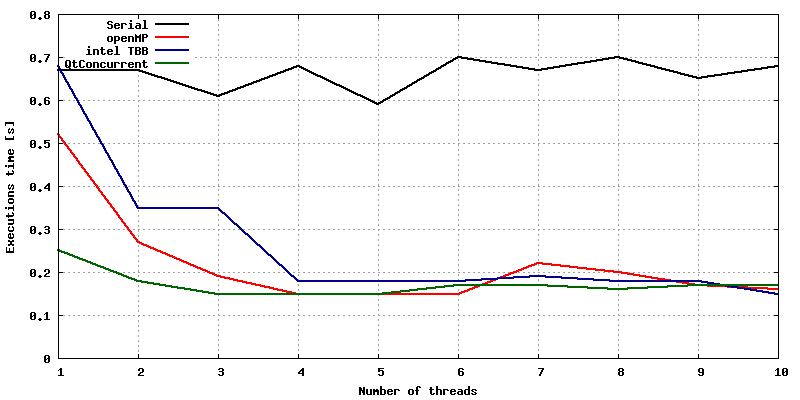
\includegraphics[height=5cm]{reduce.png} 
\end{center}

\begin{exampleblock}{Note}
\small
No need for more than 4 threads.
\end{exampleblock}

\end{frame}

\subsection{Sort}

%----------- slide --------------------------------------------------%


\begin{frame}[fragile]{Serial sort}

\begin{block}{c++ code}

\tiny
\begin{Verbatim}[commandchars=\\\{\},numbers=left,firstnumber=1,stepnumber=1]
\PY{k+kt}{void} \PY{n}{serialSort}\PY{p}{(}\PY{n}{std}\PY{o}{:}\PY{o}{:}\PY{n}{vector}\PY{o}{<}\PY{k+kt}{float}\PY{o}{>}\PY{o}{&} \PY{n}{data}\PY{p}{)}
\PY{p}{\PYZob{}}
  \PY{n}{std}\PY{o}{:}\PY{o}{:}\PY{n}{sort}\PY{p}{(}\PY{n}{data}\PY{p}{.}\PY{n}{begin}\PY{p}{(}\PY{p}{)}\PY{p}{,} \PY{n}{data}\PY{p}{.}\PY{n}{end}\PY{p}{(}\PY{p}{)}\PY{p}{)}\PY{p}{;}
\PY{p}{\PYZcb{}}
\end{Verbatim}

\end{block}

\begin{exampleblock}{Note: quicksort}
  \small
  \begin{itemize}
    \item Pick a pivot point.
    \item Partition: Swap elements compared to pivot point.
    \item Recursively calls itself with the 2 new partitions.
  \end{itemize}
\end{exampleblock}

\end{frame}

%----------- slide --------------------------------------------------%


\begin{frame}[fragile]{openMP, Intel TBB sort}

\begin{block}{openMP c++ code}

\tiny
\begin{Verbatim}[commandchars=\\\{\},numbers=left,firstnumber=1,stepnumber=1]
\PY{c+cp}{\PYZsh{}}\PY{c+cp}{include <parallel}\PY{c+cp}{/}\PY{c+cp}{algorithm>}

\PY{k+kt}{void} \PY{n}{openMpSort}\PY{p}{(}\PY{n}{std}\PY{o}{:}\PY{o}{:}\PY{n}{vector}\PY{o}{<}\PY{k+kt}{float}\PY{o}{>}\PY{o}{&} \PY{n}{data}\PY{p}{)}
\PY{p}{\PYZob{}}
  \PY{n}{\PYZus{}\PYZus{}gnu\PYZus{}parallel}\PY{o}{:}\PY{o}{:}\PY{n}{sort}\PY{p}{(}\PY{n}{data}\PY{p}{.}\PY{n}{begin}\PY{p}{(}\PY{p}{)}\PY{p}{,} \PY{n}{data}\PY{p}{.}\PY{n}{end}\PY{p}{(}\PY{p}{)}\PY{p}{)}\PY{p}{;}
\PY{p}{\PYZcb{}}
\end{Verbatim}

\end{block}

\begin{exampleblock}{Note}
\small
Some algorithms are already rewritten to work in parallel with openMP.
\end{exampleblock}

\begin{block}{Intel TBB c++ code}

\tiny
\begin{Verbatim}[commandchars=\\\{\},numbers=left,firstnumber=1,stepnumber=1]
\PY{k+kt}{void} \PY{n}{itbbSort}\PY{p}{(}\PY{n}{std}\PY{o}{:}\PY{o}{:}\PY{n}{vector}\PY{o}{<}\PY{k+kt}{float}\PY{o}{>}\PY{o}{&} \PY{n}{data}\PY{p}{)}
\PY{p}{\PYZob{}}
  \PY{n}{tbb}\PY{o}{:}\PY{o}{:}\PY{n}{parallel\PYZus{}sort}\PY{p}{(}\PY{n}{data}\PY{p}{.}\PY{n}{begin}\PY{p}{(}\PY{p}{)}\PY{p}{,} \PY{n}{data}\PY{p}{.}\PY{n}{end}\PY{p}{(}\PY{p}{)}\PY{p}{)}\PY{p}{;}
\PY{p}{\PYZcb{}}
\end{Verbatim}

\end{block}

\end{frame}

%----------- slide --------------------------------------------------%

\begin{frame}[fragile]{Sort execution times}

\begin{center}
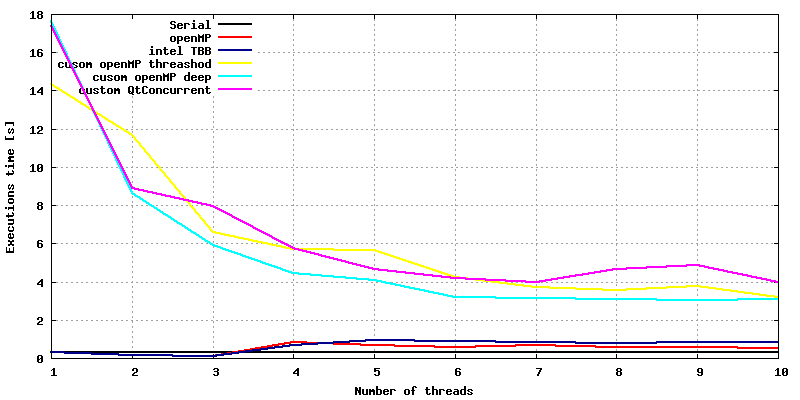
\includegraphics[height=5cm]{sort1.png} 
\end{center}

\begin{exampleblock}{Note}
\small
No need for more than 6 threads.
\end{exampleblock}

\end{frame}

%----------- slide --------------------------------------------------%


\begin{frame}[fragile]{Custom QtConcurrent sort}

\begin{block}{c++ code}

\tiny
\begin{Verbatim}[commandchars=\\\{\},numbers=left,firstnumber=1,stepnumber=1]
\PY{k}{template} \PY{o}{<}\PY{k}{class} \PY{n+nc}{SortType}\PY{o}{>}
\PY{k+kt}{long} \PY{n}{QsPartition}\PY{p}{(}\PY{n}{SortType} \PY{n}{outputArray}\PY{p}{[}\PY{p}{]}\PY{p}{,} \PY{k+kt}{long} \PY{n}{left}\PY{p}{,} \PY{k+kt}{long} \PY{n}{right}\PY{p}{)} \PY{p}{\PYZob{}} \PY{p}{.}\PY{p}{.}\PY{p}{.} \PY{p}{\PYZcb{}}

\PY{k}{template} \PY{o}{<}\PY{k}{class} \PY{n+nc}{SortType}\PY{o}{>}
\PY{k+kt}{void} \PY{n}{QsSequential}\PY{p}{(}\PY{n}{SortType} \PY{n}{array}\PY{p}{[}\PY{p}{]}\PY{p}{,} \PY{k}{const} \PY{k+kt}{long} \PY{n}{left}\PY{p}{,} \PY{k}{const} \PY{k+kt}{long} \PY{n}{right}\PY{p}{)} \PY{p}{\PYZob{}} \PY{p}{.}\PY{p}{.}\PY{p}{.} \PY{p}{\PYZcb{}}

\PY{k}{template} \PY{o}{<}\PY{k}{class} \PY{n+nc}{SortType}\PY{o}{>}
\PY{k+kt}{void} \PY{n}{QuickSortTask} \PY{p}{(}\PY{n}{SortType} \PY{n}{array}\PY{p}{[}\PY{p}{]}\PY{p}{,} \PY{k}{const} \PY{k+kt}{long} \PY{n}{left}\PY{p}{,} \PY{k}{const} \PY{k+kt}{long} \PY{n}{right}\PY{p}{,} \PY{k}{const} \PY{k+kt}{int} \PY{n}{deep}\PY{p}{)}
\PY{p}{\PYZob{}}
  \PY{k}{if} \PY{p}{(}\PY{n}{left} \PY{o}{<} \PY{n}{right}\PY{p}{)} \PY{p}{\PYZob{}}
    \PY{k}{if} \PY{p}{(}\PY{n}{deep}\PY{p}{)} \PY{p}{\PYZob{}}
      \PY{k}{const} \PY{k+kt}{long} \PY{n}{part} \PY{o}{=} \PY{n}{QsPartition}\PY{p}{(}\PY{n}{array}\PY{p}{,} \PY{n}{left}\PY{p}{,} \PY{n}{right}\PY{p}{)}\PY{p}{;}
      \PY{n}{QtConcurrent}\PY{o}{:}\PY{o}{:}\PY{n}{run}\PY{p}{(}\PY{n}{QuickSortTask}\PY{o}{<}\PY{n}{SortType}\PY{o}{>}\PY{p}{,} \PY{n}{array}\PY{p}{,} \PY{n}{part} \PY{o}{+} \PY{l+m+mi}{1}\PY{p}{,} \PY{n}{right}\PY{p}{,} \PY{n}{deep} \PY{o}{-} \PY{l+m+mi}{1}\PY{p}{)}\PY{p}{;}
      \PY{n}{QtConcurrent}\PY{o}{:}\PY{o}{:}\PY{n}{run}\PY{p}{(}\PY{n}{QuickSortTask}\PY{o}{<}\PY{n}{SortType}\PY{o}{>}\PY{p}{,} \PY{n}{array}\PY{p}{,} \PY{n}{left}\PY{p}{,} \PY{n}{part} \PY{o}{-} \PY{l+m+mi}{1}\PY{p}{,} \PY{n}{deep} \PY{o}{-} \PY{l+m+mi}{1}\PY{p}{)}\PY{p}{;}
    \PY{p}{\PYZcb{}} \PY{k}{else} \PY{p}{\PYZob{}}
      \PY{k}{const} \PY{k+kt}{long} \PY{n}{part} \PY{o}{=} \PY{n}{QsPartition}\PY{p}{(}\PY{n}{array}\PY{p}{,} \PY{n}{left}\PY{p}{,} \PY{n}{right}\PY{p}{)}\PY{p}{;}
      \PY{n}{QsSequential}\PY{p}{(}\PY{n}{array}\PY{p}{,}\PY{n}{part} \PY{o}{+} \PY{l+m+mi}{1}\PY{p}{,}\PY{n}{right}\PY{p}{)}\PY{p}{;}
      \PY{n}{QsSequential}\PY{p}{(}\PY{n}{array}\PY{p}{,}\PY{n}{left}\PY{p}{,}\PY{n}{part} \PY{o}{-} \PY{l+m+mi}{1}\PY{p}{)}\PY{p}{;}
    \PY{p}{\PYZcb{}}
  \PY{p}{\PYZcb{}}
\PY{p}{\PYZcb{}}

\PY{k+kt}{void} \PY{n}{QtSort}\PY{p}{(}\PY{n}{std}\PY{o}{:}\PY{o}{:}\PY{n}{vector}\PY{o}{<}\PY{k+kt}{float}\PY{o}{>}\PY{o}{&} \PY{n}{data}\PY{p}{)}
\PY{p}{\PYZob{}}
  \PY{n}{QtConcurrent}\PY{o}{:}\PY{o}{:}\PY{n}{run}\PY{p}{(}\PY{n}{QuickSortTask}\PY{o}{<}\PY{k+kt}{float}\PY{o}{>}\PY{p}{,} \PY{n}{data}\PY{p}{.}\PY{n}{data}\PY{p}{(}\PY{p}{)}\PY{p}{,} \PY{l+m+mi}{0}\PY{p}{,} \PY{n}{data}\PY{p}{.}\PY{n}{size}\PY{p}{(}\PY{p}{)} \PY{o}{-} \PY{l+m+mi}{1}\PY{p}{,} \PY{l+m+mi}{6}\PY{p}{)}\PY{p}{;}
  \PY{n}{QThreadPool}\PY{o}{:}\PY{o}{:}\PY{n}{globalInstance}\PY{p}{(}\PY{p}{)}\PY{o}{-}\PY{o}{>}\PY{n}{waitForDone}\PY{p}{(}\PY{p}{)}\PY{p}{;}
\PY{p}{\PYZcb{}}
\end{Verbatim}

\end{block}

\end{frame}

%----------- slide --------------------------------------------------%


\begin{frame}[fragile]{Custom openMP sort}

\begin{block}{c++ code}

\tiny
\begin{Verbatim}[commandchars=\\\{\},numbers=left,firstnumber=1,stepnumber=1]
\PY{k+kt}{void} \PY{n}{sample\PYZus{}qsort}\PY{p}{(}\PY{k+kt}{float}\PY{o}{*} \PY{n}{begin}\PY{p}{,} \PY{k+kt}{float}\PY{o}{*} \PY{n}{end}\PY{p}{)} \PY{p}{\PYZob{}} \PY{p}{.}\PY{p}{.}\PY{p}{.} \PY{p}{\PYZcb{}}

\PY{k+kt}{void} \PY{n}{sample\PYZus{}qsort\PYZus{}serial}\PY{p}{(}\PY{k+kt}{float}\PY{o}{*} \PY{n}{begin}\PY{p}{,} \PY{k+kt}{float}\PY{o}{*} \PY{n}{end}\PY{p}{)} \PY{p}{\PYZob{}} \PY{p}{.}\PY{p}{.}\PY{p}{.} \PY{p}{\PYZcb{}}

\PY{k+kt}{void} \PY{n}{sample\PYZus{}qsort\PYZus{}adaptive}\PY{p}{(}\PY{k+kt}{float}\PY{o}{*} \PY{n}{begin}\PY{p}{,} \PY{k+kt}{float}\PY{o}{*} \PY{n}{end}\PY{p}{,} \PY{k}{const} \PY{k+kt}{long} \PY{n}{nthreshold}\PY{p}{)}
\PY{p}{\PYZob{}}
  \PY{k}{if} \PY{p}{(}\PY{n}{begin} \PY{o}{!}\PY{o}{=} \PY{n}{end}\PY{p}{)} \PY{p}{\PYZob{}}
    \PY{c+c1}{// parition ...}
    \PY{k}{if} \PY{p}{(}\PY{n}{end} \PY{o}{-} \PY{n}{begin} \PY{o}{+} \PY{l+m+mi}{1} \PY{o}{<}\PY{o}{=} \PY{n}{nthreshold}\PY{p}{)} \PY{p}{\PYZob{}}
      \PY{n}{sample\PYZus{}qsort\PYZus{}serial}\PY{p}{(}\PY{n}{begin}\PY{p}{,} \PY{n}{middle}\PY{p}{)}\PY{p}{;}
      \PY{n}{sample\PYZus{}qsort\PYZus{}serial}\PY{p}{(}\PY{o}{+}\PY{o}{+}\PY{n}{middle}\PY{p}{,} \PY{o}{+}\PY{o}{+}\PY{n}{end}\PY{p}{)}\PY{p}{;}
    \PY{p}{\PYZcb{}} \PY{k}{else} \PY{p}{\PYZob{}}
\PY{c+cp}{\PYZsh{}}\PY{c+cp}{pragma omp task}
      \PY{n}{sample\PYZus{}qsort\PYZus{}adaptive}\PY{p}{(}\PY{n}{begin}\PY{p}{,} \PY{n}{middle}\PY{p}{,} \PY{n}{nthreshold}\PY{p}{)}\PY{p}{;}
\PY{c+cp}{\PYZsh{}}\PY{c+cp}{pragma omp task}
      \PY{n}{sample\PYZus{}qsort\PYZus{}adaptive}\PY{p}{(}\PY{o}{+}\PY{o}{+}\PY{n}{middle}\PY{p}{,} \PY{o}{+}\PY{o}{+}\PY{n}{end}\PY{p}{,} \PY{n}{nthreshold}\PY{p}{)}\PY{p}{;}
    \PY{p}{\PYZcb{}}
  \PY{p}{\PYZcb{}}
\PY{p}{\PYZcb{}}

\PY{k+kt}{void} \PY{n}{sample\PYZus{}qsort\PYZus{}adaptive}\PY{p}{(}\PY{k+kt}{float}\PY{o}{*} \PY{n}{begin}\PY{p}{,} \PY{k+kt}{float}\PY{o}{*} \PY{n}{end}\PY{p}{)}
\PY{p}{\PYZob{}}
  \PY{k+kt}{long} \PY{n}{nthreshold} \PY{o}{=} \PY{n}{ceil}\PY{p}{(}\PY{n}{sqrt}\PY{p}{(}\PY{n}{end} \PY{o}{-} \PY{n}{begin} \PY{o}{+} \PY{l+m+mi}{1}\PY{p}{)}\PY{p}{)} \PY{o}{/} \PY{l+m+mi}{2}\PY{p}{;}
\PY{c+cp}{\PYZsh{}}\PY{c+cp}{pragma omp parallel}
\PY{c+cp}{\PYZsh{}}\PY{c+cp}{pragma omp single nowait}
  \PY{n}{sample\PYZus{}qsort\PYZus{}adaptive}\PY{p}{(}\PY{n}{begin}\PY{p}{,} \PY{n}{end}\PY{p}{,} \PY{n}{nthreshold}\PY{p}{)}\PY{p}{;}
\PY{p}{\PYZcb{}}
\end{Verbatim}

\end{block}

\end{frame}

%----------- slide --------------------------------------------------%

\begin{frame}[fragile]{Sort times of custom algorithms}

\begin{center}
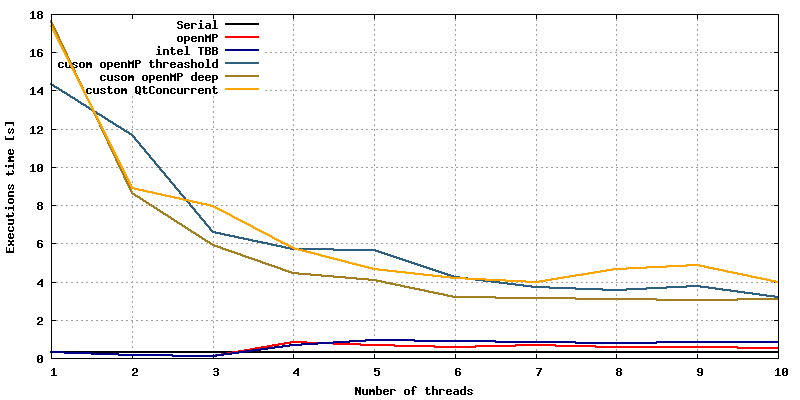
\includegraphics[height=5cm]{sort2.png} 
\end{center}


\begin{exampleblock}{Note}
\small
Container size is 6M - miserable...
\end{exampleblock}

\end{frame}

%----------- slide --------------------------------------------------%


\begin{frame}[fragile]{Two quicksort approach to }

\begin{columns}[t]

\column{1.7in}
\begin{block}{Treshold}
\tiny
\begin{Verbatim}[commandchars=\\\{\},numbers=left,firstnumber=1,stepnumber=1]
\PY{k+kt}{void} \PY{n}{qsort}\PY{p}{(}\PY{k+kt}{float}\PY{o}{*} \PY{n}{begin}\PY{p}{,}
           \PY{k+kt}{float}\PY{o}{*} \PY{n}{end}\PY{p}{,}
           \PY{k}{const} \PY{k+kt}{long} \PY{n}{nthreshold}\PY{p}{)}
\PY{p}{\PYZob{}}
  \PY{k}{if} \PY{p}{(}\PY{n}{begin} \PY{o}{!}\PY{o}{=} \PY{n}{end}\PY{p}{)} \PY{p}{\PYZob{}}
    \PY{c+c1}{// parition ...}
    \PY{k}{if} \PY{p}{(}\PY{n}{end}\PY{o}{-}\PY{n}{begin}\PY{o}{+}\PY{l+m+mi}{1} \PY{o}{<}\PY{o}{=} \PY{n}{nthreshold}\PY{p}{)} \PY{p}{\PYZob{}}
      \PY{c+c1}{// serial sort ...}
    \PY{p}{\PYZcb{}} \PY{k}{else} \PY{p}{\PYZob{}}
      \PY{c+c1}{// parallel sort ...}
    \PY{p}{\PYZcb{}}
  \PY{p}{\PYZcb{}}
\PY{p}{\PYZcb{}}

\PY{k+kt}{long} \PY{n}{deep} \PY{o}{=}
  \PY{n}{ceil}\PY{p}{(}\PY{n}{sqrt}\PY{p}{(}\PY{n}{end} \PY{o}{-} \PY{n}{begin} \PY{o}{+} \PY{l+m+mi}{1}\PY{p}{)}\PY{p}{)} \PY{o}{/} \PY{l+m+mi}{2}\PY{p}{;}
\end{Verbatim}

\end{block}

\column{1.5in}
\begin{block}{Depth}
\tiny
\begin{Verbatim}[commandchars=\\\{\},numbers=left,firstnumber=1,stepnumber=1]
\PY{k+kt}{void} \PY{n}{qsort}\PY{p}{(}\PY{k+kt}{float}\PY{o}{*} \PY{n}{begin}\PY{p}{,}
           \PY{k+kt}{float}\PY{o}{*} \PY{n}{end}\PY{p}{,}
           \PY{k}{const} \PY{k+kt}{int} \PY{n}{deep}\PY{p}{)}
\PY{p}{\PYZob{}}
  \PY{k}{if} \PY{p}{(}\PY{n}{begin} \PY{o}{!}\PY{o}{=} \PY{n}{end}\PY{p}{)} \PY{p}{\PYZob{}}
    \PY{c+c1}{// parition ...}
    \PY{k}{if} \PY{p}{(}\PY{n}{deep}\PY{p}{)} \PY{p}{\PYZob{}}
      \PY{c+c1}{// serial sort ...}
    \PY{p}{\PYZcb{}} \PY{k}{else} \PY{p}{\PYZob{}}
      \PY{c+c1}{// parallel sort with deep-1}
    \PY{p}{\PYZcb{}}
  \PY{p}{\PYZcb{}}
\PY{p}{\PYZcb{}}

\PY{k+kt}{long} \PY{n}{deep} \PY{o}{=} \PY{l+m+mi}{15}\PY{p}{;}
\end{Verbatim}
\end{block}


\end{columns}

\begin{exampleblock}{Note}
\small
Depth seems simpler yet faster.
\end{exampleblock}

\end{frame}


\section{Final thoughts}


%----------- slide --------------------------------------------------%

\subsection{Grainsize}

%----------- slide --------------------------------------------------%

\begin{frame}[fragile]{Chunk size}

\begin{center}
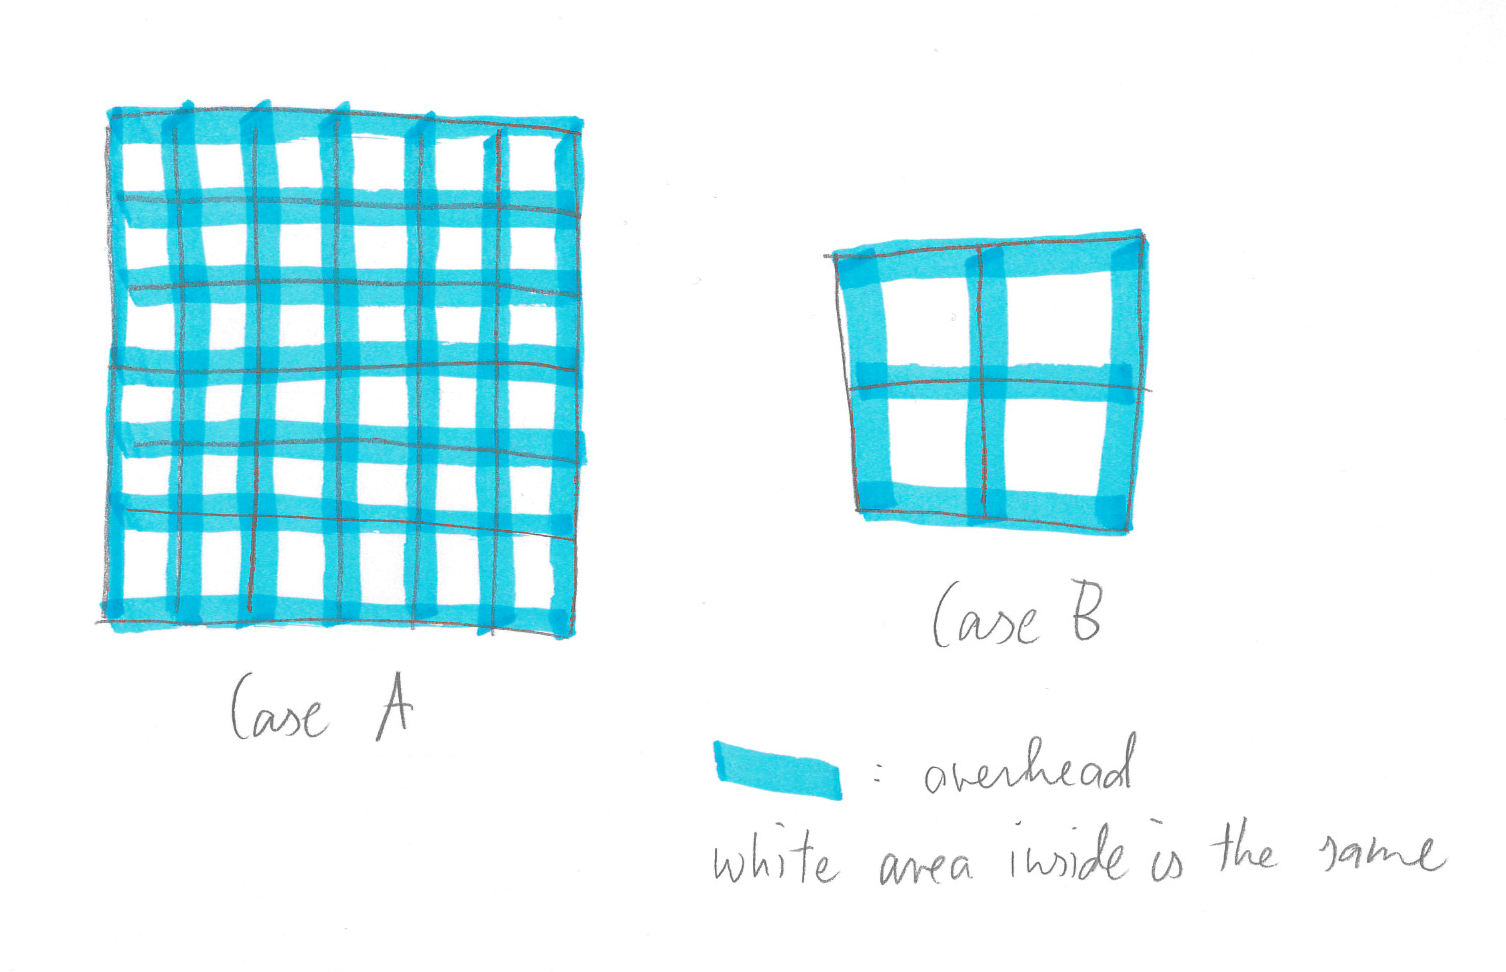
\includegraphics[height=5cm]{chunksize.png}  
\end{center}

\begin{exampleblock}{Note}
\small
\begin{itemize}
 \item Unit is loop interaction per chunk. Default value is 1.
 \item Too small chunks can introduce more overhead than useful work.
\end{itemize}
\end{exampleblock}

\end{frame}

%----------- slide --------------------------------------------------%

\begin{frame}[fragile]{Grain size}

\begin{center}
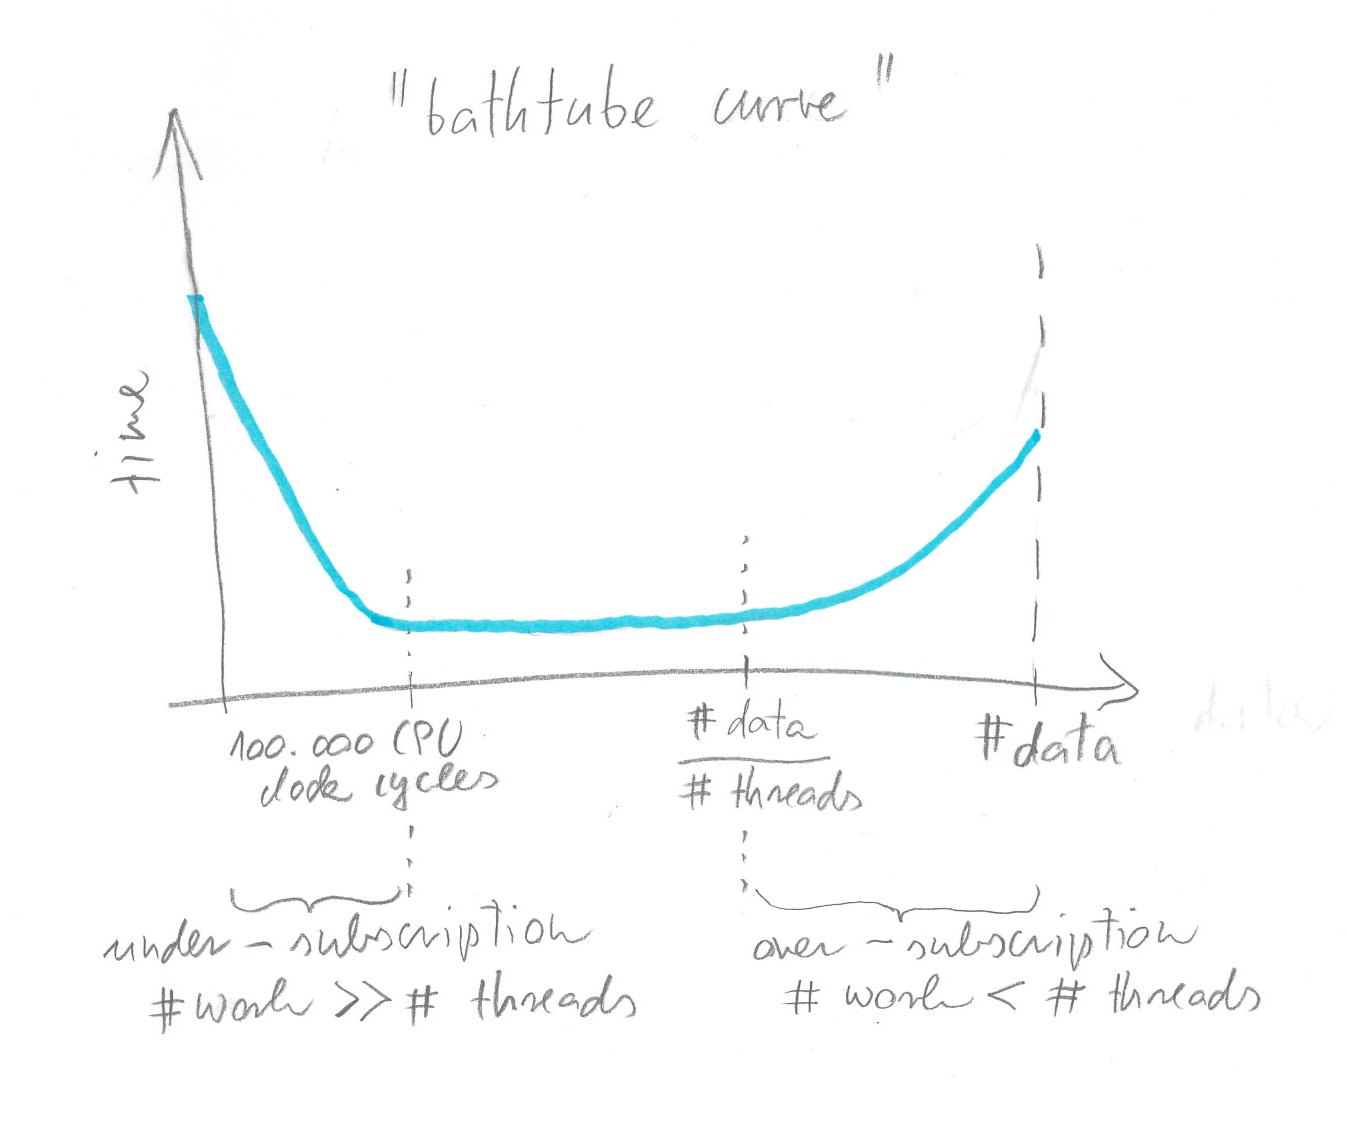
\includegraphics[height=5cm]{grainsize.png}  
\end{center}

\begin{exampleblock}{Note}
\small
\begin{itemize}
 \item Unit is CPU cycles.
 \item Should be at least ~100.000.
\end{itemize}
\end{exampleblock}

\end{frame}

%----------- slide --------------------------------------------------%

\begin{frame}[fragile]{Task stealing - Intel TBB}

\begin{block}{Task stealing}
\begin{itemize}
  \item Each thread has a queue of tasks.
  \item If a thread has no more tasks then it ``steals'' from another.
  \item Think about tasks, not about threads when programming.
\end{itemize}
\end{block}

\begin{exampleblock}{Threadpool}
A threadpool with a commond concurrent queue of tasks is a common practice in networking servers.
\end{exampleblock}

\begin{exampleblock}{Work stealing}
Another implementation is Cilk\cite{cilk} - where each processor has a stack of frames.
\end{exampleblock}


\end{frame}


\subsection{Convolution}

%----------- slide --------------------------------------------------%

\begin{frame}[fragile]{1D gaussian filter}

\begin{columns}[t]

\column{2.5in}

\begin{block}{c++ code}

\tiny
\begin{Verbatim}[commandchars=\\\{\},numbers=left,firstnumber=1,stepnumber=1]
\PY{k+kt}{void} \PY{n}{serialConvolution}\PY{p}{(}\PY{n}{std}\PY{o}{:}\PY{o}{:}\PY{n}{vector}\PY{o}{<}\PY{k+kt}{float}\PY{o}{>}\PY{o}{&} \PY{n}{output}\PY{p}{,}
                       \PY{k}{const} \PY{n}{std}\PY{o}{:}\PY{o}{:}\PY{n}{vector}\PY{o}{<}\PY{k+kt}{float}\PY{o}{>}\PY{o}{&} \PY{n}{input}\PY{p}{,}
                       \PY{k}{const} \PY{n}{std}\PY{o}{:}\PY{o}{:}\PY{n}{vector}\PY{o}{<}\PY{k+kt}{float}\PY{o}{>}\PY{o}{&} \PY{n}{kernel}\PY{p}{)}
\PY{p}{\PYZob{}}
  \PY{c+c1}{// skipping the edges: separate loops, paddings}
  \PY{c+c1}{// output.size == input.size()-kernel.size()-1;}

  \PY{k}{for} \PY{p}{(}\PY{n}{size\PYZus{}t} \PY{n}{i} \PY{o}{=} \PY{l+m+mi}{0}\PY{p}{;} \PY{n}{i} \PY{o}{<} \PY{n}{output}\PY{p}{.}\PY{n}{size}\PY{p}{(}\PY{p}{)}\PY{p}{;} \PY{n}{i}\PY{o}{+}\PY{o}{+}\PY{p}{)} \PY{p}{\PYZob{}}
    \PY{k+kt}{float} \PY{n}{sum} \PY{o}{=} \PY{l+m+mi}{0}\PY{p}{;}
    \PY{k}{for} \PY{p}{(}\PY{n}{size\PYZus{}t} \PY{n}{j} \PY{o}{=} \PY{l+m+mi}{0}\PY{p}{;} \PY{n}{j} \PY{o}{<}\PY{o}{=} \PY{n}{kernel}\PY{p}{.}\PY{n}{size}\PY{p}{(}\PY{p}{)}\PY{p}{;} \PY{n}{j}\PY{o}{+}\PY{o}{+}\PY{p}{)}
      \PY{n}{sum} \PY{o}{+}\PY{o}{=} \PY{n}{input}\PY{p}{[}\PY{n}{i}\PY{o}{+}\PY{n}{j}\PY{p}{]} \PY{o}{*} \PY{n}{kernel}\PY{p}{[}\PY{n}{j}\PY{p}{]}\PY{p}{;}

    \PY{n}{output}\PY{p}{[}\PY{n}{i}\PY{p}{]} \PY{o}{=} \PY{n}{sum}\PY{p}{;}
  \PY{p}{\PYZcb{}}
\PY{p}{\PYZcb{}}
\end{Verbatim}


\end{block}

\column{1.5in}

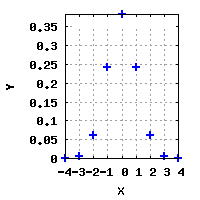
\includegraphics[height=3cm]{1d_gauss.png} 

\end{columns}

\begin{exampleblock}{Note}
\tiny
\verb|float kernel[7] = { 0.06, 0.061, 0.242, 0.383, 0.242, 0.061, 0.06 }|
\end{exampleblock}

\end{frame}


%----------- slide --------------------------------------------------%


\begin{frame}[fragile]{Optimized convolution}

\begin{block}{c++ code}

\tiny
\begin{Verbatim}[commandchars=\\\{\},numbers=left,firstnumber=1,stepnumber=1]
\PY{k+kt}{void} \PY{k}{operator}\PY{p}{(}\PY{p}{)}\PY{p}{(}\PY{k}{const} \PY{n}{tbb}\PY{o}{:}\PY{o}{:}\PY{n}{blocked\PYZus{}range}\PY{o}{<}\PY{n}{size\PYZus{}t}\PY{o}{>}\PY{o}{&} \PY{n}{r}\PY{p}{)} \PY{k}{const}
\PY{p}{\PYZob{}}
  \PY{c+c1}{// skipping the edges, shall be done in separate task}
  \PY{k}{const} \PY{k+kt}{float}\PY{o}{*} \PY{n}{p} \PY{o}{=} \PY{o}{&}\PY{n}{m\PYZus{}input}\PY{p}{[}\PY{l+m+mi}{0}\PY{p}{]} \PY{o}{+} \PY{n}{r}\PY{p}{.}\PY{n}{begin}\PY{p}{(}\PY{p}{)}\PY{p}{;}
  \PY{k+kt}{float}\PY{o}{*} \PY{n}{d} \PY{o}{=} \PY{o}{&}\PY{n}{m\PYZus{}output}\PY{p}{[}\PY{l+m+mi}{0}\PY{p}{]} \PY{o}{+} \PY{n}{r}\PY{p}{.}\PY{n}{begin}\PY{p}{(}\PY{p}{)}\PY{p}{;}

  \PY{k}{const} \PY{n}{size\PYZus{}t} \PY{n}{n} \PY{o}{=} \PY{n}{m\PYZus{}kernel}\PY{p}{.}\PY{n}{size}\PY{p}{(}\PY{p}{)}\PY{p}{;}
  \PY{k+kt}{float} \PY{n}{k}\PY{p}{[}\PY{n}{n}\PY{p}{]}\PY{p}{;} \PY{c+c1}{// pre-read kernel}
  \PY{k+kt}{float} \PY{n}{c}\PY{p}{[}\PY{n}{n}\PY{p}{]}\PY{p}{;} \PY{c+c1}{// pre-read values}
  \PY{n}{k}\PY{p}{[}\PY{l+m+mi}{0}\PY{p}{]} \PY{o}{=} \PY{n}{m\PYZus{}kernel}\PY{p}{[}\PY{l+m+mi}{0}\PY{p}{]}\PY{p}{;}
  \PY{k}{for} \PY{p}{(}\PY{n}{size\PYZus{}t} \PY{n}{i} \PY{o}{=} \PY{l+m+mi}{1}\PY{p}{;} \PY{n}{i} \PY{o}{<} \PY{n}{n}\PY{p}{;} \PY{o}{+}\PY{o}{+}\PY{n}{i}\PY{p}{)} \PY{p}{\PYZob{}}
    \PY{n}{c}\PY{p}{[}\PY{n}{i}\PY{p}{]} \PY{o}{=} \PY{n}{m\PYZus{}input}\PY{p}{[}\PY{n}{i}\PY{o}{-}\PY{l+m+mi}{1}\PY{p}{]}\PY{p}{;}
    \PY{n}{k}\PY{p}{[}\PY{n}{i}\PY{p}{]} \PY{o}{=} \PY{n}{m\PYZus{}kernel}\PY{p}{[}\PY{n}{i}\PY{p}{]}\PY{p}{;}
  \PY{p}{\PYZcb{}}

  \PY{c+c1}{// chunk size \PYZpc{} kernel.size() != 0 should be handled...}
  \PY{k}{for} \PY{p}{(}\PY{n}{size\PYZus{}t} \PY{n}{i} \PY{o}{=} \PY{l+m+mi}{0}\PY{p}{;} \PY{n}{i} \PY{o}{<} \PY{n}{r}\PY{p}{.}\PY{n}{size}\PY{p}{(}\PY{p}{)}\PY{p}{;} \PY{n}{i} \PY{o}{+}\PY{o}{=} \PY{n}{n}\PY{p}{)} \PY{p}{\PYZob{}}
    \PY{n}{d}\PY{p}{[}\PY{n}{i}\PY{o}{+}\PY{l+m+mi}{0}\PY{p}{]} \PY{o}{=} \PY{p}{(}\PY{n}{c}\PY{p}{[}\PY{l+m+mi}{0}\PY{p}{]} \PY{o}{=} \PY{n}{p}\PY{p}{[}\PY{n}{i}\PY{o}{+}\PY{l+m+mi}{0}\PY{p}{]}\PY{p}{)}\PY{o}{*}\PY{n}{k}\PY{p}{[}\PY{l+m+mi}{0}\PY{p}{]}\PY{o}{+}\PY{n}{c}\PY{p}{[}\PY{l+m+mi}{1}\PY{p}{]}\PY{o}{*}\PY{n}{k}\PY{p}{[}\PY{l+m+mi}{2}\PY{p}{]}\PY{o}{+}\PY{n}{c}\PY{p}{[}\PY{l+m+mi}{2}\PY{p}{]}\PY{o}{*}\PY{n}{k}\PY{p}{[}\PY{l+m+mi}{2}\PY{p}{]}\PY{o}{+}\PY{n}{c}\PY{p}{[}\PY{l+m+mi}{3}\PY{p}{]}\PY{o}{*}\PY{n}{k}\PY{p}{[}\PY{l+m+mi}{3}\PY{p}{]}\PY{o}{+}\PY{n}{c}\PY{p}{[}\PY{l+m+mi}{4}\PY{p}{]}\PY{o}{*}\PY{n}{k}\PY{p}{[}\PY{l+m+mi}{4}\PY{p}{]}\PY{o}{+}\PY{n}{c}\PY{p}{[}\PY{l+m+mi}{5}\PY{p}{]}\PY{o}{*}\PY{n}{k}\PY{p}{[}\PY{l+m+mi}{5}\PY{p}{]}\PY{o}{+}\PY{n}{c}\PY{p}{[}\PY{l+m+mi}{6}\PY{p}{]}\PY{o}{*}\PY{n}{k}\PY{p}{[}\PY{l+m+mi}{6}\PY{p}{]}\PY{p}{;}
    \PY{n}{d}\PY{p}{[}\PY{n}{i}\PY{o}{+}\PY{l+m+mi}{1}\PY{p}{]} \PY{o}{=} \PY{p}{(}\PY{n}{c}\PY{p}{[}\PY{l+m+mi}{6}\PY{p}{]} \PY{o}{=} \PY{n}{p}\PY{p}{[}\PY{n}{i}\PY{o}{+}\PY{l+m+mi}{1}\PY{p}{]}\PY{p}{)}\PY{o}{*}\PY{n}{k}\PY{p}{[}\PY{l+m+mi}{0}\PY{p}{]}\PY{o}{+}\PY{n}{c}\PY{p}{[}\PY{l+m+mi}{0}\PY{p}{]}\PY{o}{*}\PY{n}{k}\PY{p}{[}\PY{l+m+mi}{2}\PY{p}{]}\PY{o}{+}\PY{n}{c}\PY{p}{[}\PY{l+m+mi}{1}\PY{p}{]}\PY{o}{*}\PY{n}{k}\PY{p}{[}\PY{l+m+mi}{2}\PY{p}{]}\PY{o}{+}\PY{n}{c}\PY{p}{[}\PY{l+m+mi}{2}\PY{p}{]}\PY{o}{*}\PY{n}{k}\PY{p}{[}\PY{l+m+mi}{3}\PY{p}{]}\PY{o}{+}\PY{n}{c}\PY{p}{[}\PY{l+m+mi}{3}\PY{p}{]}\PY{o}{*}\PY{n}{k}\PY{p}{[}\PY{l+m+mi}{4}\PY{p}{]}\PY{o}{+}\PY{n}{c}\PY{p}{[}\PY{l+m+mi}{4}\PY{p}{]}\PY{o}{*}\PY{n}{k}\PY{p}{[}\PY{l+m+mi}{5}\PY{p}{]}\PY{o}{+}\PY{n}{c}\PY{p}{[}\PY{l+m+mi}{5}\PY{p}{]}\PY{o}{*}\PY{n}{k}\PY{p}{[}\PY{l+m+mi}{6}\PY{p}{]}\PY{p}{;}
    \PY{n}{d}\PY{p}{[}\PY{n}{i}\PY{o}{+}\PY{l+m+mi}{2}\PY{p}{]} \PY{o}{=} \PY{p}{(}\PY{n}{c}\PY{p}{[}\PY{l+m+mi}{5}\PY{p}{]} \PY{o}{=} \PY{n}{p}\PY{p}{[}\PY{n}{i}\PY{o}{+}\PY{l+m+mi}{2}\PY{p}{]}\PY{p}{)}\PY{o}{*}\PY{n}{k}\PY{p}{[}\PY{l+m+mi}{0}\PY{p}{]}\PY{o}{+}\PY{n}{c}\PY{p}{[}\PY{l+m+mi}{6}\PY{p}{]}\PY{o}{*}\PY{n}{k}\PY{p}{[}\PY{l+m+mi}{2}\PY{p}{]}\PY{o}{+}\PY{n}{c}\PY{p}{[}\PY{l+m+mi}{0}\PY{p}{]}\PY{o}{*}\PY{n}{k}\PY{p}{[}\PY{l+m+mi}{2}\PY{p}{]}\PY{o}{+}\PY{n}{c}\PY{p}{[}\PY{l+m+mi}{1}\PY{p}{]}\PY{o}{*}\PY{n}{k}\PY{p}{[}\PY{l+m+mi}{3}\PY{p}{]}\PY{o}{+}\PY{n}{c}\PY{p}{[}\PY{l+m+mi}{2}\PY{p}{]}\PY{o}{*}\PY{n}{k}\PY{p}{[}\PY{l+m+mi}{4}\PY{p}{]}\PY{o}{+}\PY{n}{c}\PY{p}{[}\PY{l+m+mi}{3}\PY{p}{]}\PY{o}{*}\PY{n}{k}\PY{p}{[}\PY{l+m+mi}{5}\PY{p}{]}\PY{o}{+}\PY{n}{c}\PY{p}{[}\PY{l+m+mi}{4}\PY{p}{]}\PY{o}{*}\PY{n}{k}\PY{p}{[}\PY{l+m+mi}{6}\PY{p}{]}\PY{p}{;}
    \PY{n}{d}\PY{p}{[}\PY{n}{i}\PY{o}{+}\PY{l+m+mi}{3}\PY{p}{]} \PY{o}{=} \PY{p}{(}\PY{n}{c}\PY{p}{[}\PY{l+m+mi}{4}\PY{p}{]} \PY{o}{=} \PY{n}{p}\PY{p}{[}\PY{n}{i}\PY{o}{+}\PY{l+m+mi}{3}\PY{p}{]}\PY{p}{)}\PY{o}{*}\PY{n}{k}\PY{p}{[}\PY{l+m+mi}{0}\PY{p}{]}\PY{o}{+}\PY{n}{c}\PY{p}{[}\PY{l+m+mi}{5}\PY{p}{]}\PY{o}{*}\PY{n}{k}\PY{p}{[}\PY{l+m+mi}{2}\PY{p}{]}\PY{o}{+}\PY{n}{c}\PY{p}{[}\PY{l+m+mi}{6}\PY{p}{]}\PY{o}{*}\PY{n}{k}\PY{p}{[}\PY{l+m+mi}{2}\PY{p}{]}\PY{o}{+}\PY{n}{c}\PY{p}{[}\PY{l+m+mi}{0}\PY{p}{]}\PY{o}{*}\PY{n}{k}\PY{p}{[}\PY{l+m+mi}{3}\PY{p}{]}\PY{o}{+}\PY{n}{c}\PY{p}{[}\PY{l+m+mi}{1}\PY{p}{]}\PY{o}{*}\PY{n}{k}\PY{p}{[}\PY{l+m+mi}{4}\PY{p}{]}\PY{o}{+}\PY{n}{c}\PY{p}{[}\PY{l+m+mi}{2}\PY{p}{]}\PY{o}{*}\PY{n}{k}\PY{p}{[}\PY{l+m+mi}{5}\PY{p}{]}\PY{o}{+}\PY{n}{c}\PY{p}{[}\PY{l+m+mi}{3}\PY{p}{]}\PY{o}{*}\PY{n}{k}\PY{p}{[}\PY{l+m+mi}{6}\PY{p}{]}\PY{p}{;}
    \PY{n}{d}\PY{p}{[}\PY{n}{i}\PY{o}{+}\PY{l+m+mi}{4}\PY{p}{]} \PY{o}{=} \PY{p}{(}\PY{n}{c}\PY{p}{[}\PY{l+m+mi}{3}\PY{p}{]} \PY{o}{=} \PY{n}{p}\PY{p}{[}\PY{n}{i}\PY{o}{+}\PY{l+m+mi}{4}\PY{p}{]}\PY{p}{)}\PY{o}{*}\PY{n}{k}\PY{p}{[}\PY{l+m+mi}{0}\PY{p}{]}\PY{o}{+}\PY{n}{c}\PY{p}{[}\PY{l+m+mi}{4}\PY{p}{]}\PY{o}{*}\PY{n}{k}\PY{p}{[}\PY{l+m+mi}{2}\PY{p}{]}\PY{o}{+}\PY{n}{c}\PY{p}{[}\PY{l+m+mi}{5}\PY{p}{]}\PY{o}{*}\PY{n}{k}\PY{p}{[}\PY{l+m+mi}{2}\PY{p}{]}\PY{o}{+}\PY{n}{c}\PY{p}{[}\PY{l+m+mi}{6}\PY{p}{]}\PY{o}{*}\PY{n}{k}\PY{p}{[}\PY{l+m+mi}{3}\PY{p}{]}\PY{o}{+}\PY{n}{c}\PY{p}{[}\PY{l+m+mi}{0}\PY{p}{]}\PY{o}{*}\PY{n}{k}\PY{p}{[}\PY{l+m+mi}{4}\PY{p}{]}\PY{o}{+}\PY{n}{c}\PY{p}{[}\PY{l+m+mi}{1}\PY{p}{]}\PY{o}{*}\PY{n}{k}\PY{p}{[}\PY{l+m+mi}{5}\PY{p}{]}\PY{o}{+}\PY{n}{c}\PY{p}{[}\PY{l+m+mi}{2}\PY{p}{]}\PY{o}{*}\PY{n}{k}\PY{p}{[}\PY{l+m+mi}{6}\PY{p}{]}\PY{p}{;}
    \PY{n}{d}\PY{p}{[}\PY{n}{i}\PY{o}{+}\PY{l+m+mi}{5}\PY{p}{]} \PY{o}{=} \PY{p}{(}\PY{n}{c}\PY{p}{[}\PY{l+m+mi}{2}\PY{p}{]} \PY{o}{=} \PY{n}{p}\PY{p}{[}\PY{n}{i}\PY{o}{+}\PY{l+m+mi}{5}\PY{p}{]}\PY{p}{)}\PY{o}{*}\PY{n}{k}\PY{p}{[}\PY{l+m+mi}{0}\PY{p}{]}\PY{o}{+}\PY{n}{c}\PY{p}{[}\PY{l+m+mi}{3}\PY{p}{]}\PY{o}{*}\PY{n}{k}\PY{p}{[}\PY{l+m+mi}{2}\PY{p}{]}\PY{o}{+}\PY{n}{c}\PY{p}{[}\PY{l+m+mi}{4}\PY{p}{]}\PY{o}{*}\PY{n}{k}\PY{p}{[}\PY{l+m+mi}{2}\PY{p}{]}\PY{o}{+}\PY{n}{c}\PY{p}{[}\PY{l+m+mi}{5}\PY{p}{]}\PY{o}{*}\PY{n}{k}\PY{p}{[}\PY{l+m+mi}{3}\PY{p}{]}\PY{o}{+}\PY{n}{c}\PY{p}{[}\PY{l+m+mi}{6}\PY{p}{]}\PY{o}{*}\PY{n}{k}\PY{p}{[}\PY{l+m+mi}{4}\PY{p}{]}\PY{o}{+}\PY{n}{c}\PY{p}{[}\PY{l+m+mi}{0}\PY{p}{]}\PY{o}{*}\PY{n}{k}\PY{p}{[}\PY{l+m+mi}{5}\PY{p}{]}\PY{o}{+}\PY{n}{c}\PY{p}{[}\PY{l+m+mi}{1}\PY{p}{]}\PY{o}{*}\PY{n}{k}\PY{p}{[}\PY{l+m+mi}{6}\PY{p}{]}\PY{p}{;}
    \PY{n}{d}\PY{p}{[}\PY{n}{i}\PY{o}{+}\PY{l+m+mi}{6}\PY{p}{]} \PY{o}{=} \PY{p}{(}\PY{n}{c}\PY{p}{[}\PY{l+m+mi}{1}\PY{p}{]} \PY{o}{=} \PY{n}{p}\PY{p}{[}\PY{n}{i}\PY{o}{+}\PY{l+m+mi}{6}\PY{p}{]}\PY{p}{)}\PY{o}{*}\PY{n}{k}\PY{p}{[}\PY{l+m+mi}{0}\PY{p}{]}\PY{o}{+}\PY{n}{c}\PY{p}{[}\PY{l+m+mi}{2}\PY{p}{]}\PY{o}{*}\PY{n}{k}\PY{p}{[}\PY{l+m+mi}{2}\PY{p}{]}\PY{o}{+}\PY{n}{c}\PY{p}{[}\PY{l+m+mi}{3}\PY{p}{]}\PY{o}{*}\PY{n}{k}\PY{p}{[}\PY{l+m+mi}{2}\PY{p}{]}\PY{o}{+}\PY{n}{c}\PY{p}{[}\PY{l+m+mi}{4}\PY{p}{]}\PY{o}{*}\PY{n}{k}\PY{p}{[}\PY{l+m+mi}{3}\PY{p}{]}\PY{o}{+}\PY{n}{c}\PY{p}{[}\PY{l+m+mi}{5}\PY{p}{]}\PY{o}{*}\PY{n}{k}\PY{p}{[}\PY{l+m+mi}{4}\PY{p}{]}\PY{o}{+}\PY{n}{c}\PY{p}{[}\PY{l+m+mi}{6}\PY{p}{]}\PY{o}{*}\PY{n}{k}\PY{p}{[}\PY{l+m+mi}{5}\PY{p}{]}\PY{o}{+}\PY{n}{c}\PY{p}{[}\PY{l+m+mi}{0}\PY{p}{]}\PY{o}{*}\PY{n}{k}\PY{p}{[}\PY{l+m+mi}{6}\PY{p}{]}\PY{p}{;}
  \PY{p}{\PYZcb{}}
\PY{p}{\PYZcb{}}
\end{Verbatim}


\end{block}

\end{frame}


%----------- slide --------------------------------------------------%

\begin{frame}[fragile]{Convolution running times}

\begin{center}
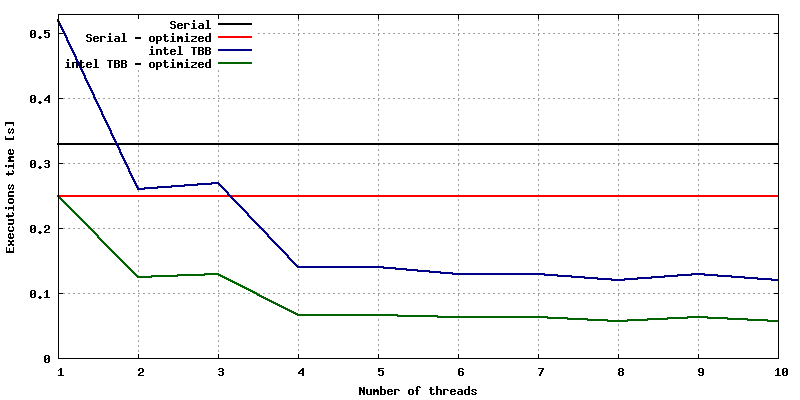
\includegraphics[height=5cm]{convolution.png}  
\end{center}


\begin{exampleblock}{Note}
\small
Memory-read optimalization can result the same performance improvements as parallelization.
\end{exampleblock}

\end{frame}

%----------- slide --------------------------------------------------%



\subsection{Summary}

\begin{frame}{Things to keep in mind}

\begin{block}{Checklist}
  \small
  \begin{itemize}
    \item Pass primitive types by value.
    \item Pass objects by address.
    \item Have function-local copies of member variables.
    \item Avoid to read values multiple times.
    \item Choose correct chunk size.
    \item Instead of shared memory, consider reduction.
    \item Plan datastructures to avoid memory-boundings.* 
  \end{itemize}
\end{block}

\pause

\begin{exampleblock}{*data-oriented design\cite{data_oriented_design}}
\small
If only someone could tell us more about it...
\end{exampleblock}

\end{frame}


\begin{frame}{Links}

\tiny
\begin{thebibliography}{100}
\bibitem{openmp}openMP.\url{http://openmp.org}
\bibitem{itbb}Intel Thread Building Blocks.\url{http://threadingbuildingblocks.org/}
\bibitem{qtconcurrent}QtConcurrent.\url{http://doc.qt.nokia.com/4.8-snapshot/qtconcurrent.html}
\bibitem{cilk}Cilk.\url{http://software.intel.com/en-us/articles/intel-cilk-plus}
\bibitem{itbb_openmp_nativethreads}Comparison of Intel TBB, openMP and native threads.\url{http://software.intel.com/en-us/articles/intel-threading-building-blocks-openmp-or-native-threads/}

\bibitem{cpp_thread}std::thread in C++\url{http://en.cppreference.com/w/cpp/thread}
\bibitem{posix_threads}POSIX threads tutorial.\url{http://www.yolinux.com/TUTORIALS/LinuxTutorialPosixThreads.html}
\bibitem{qt_thread}Qt threads.\url{http://qt-project.org/doc/qt-4.8/threads.html}

\bibitem{data_oriented_design}Data oriented design.\url{http://gamesfromwithin.com/data-oriented-design}

\bibitem{latex_beamer}\LaTeX{} beamer class for creating presentations.\url{https://bitbucket.org/rivanvx/beamer/wiki/Home}
\bibitem{gnuplot}Gnuplot - An open source plotting software.\url{http://www.gnuplot.info/}

\end{thebibliography}
\end{frame}


\end{document}